\documentclass{atistandalonetask}
\usepackage{atistandard}

\begin{document}
  \begin{atiTask}[
    title = Koordinatentransformation
  ]

Ein Koordinatensystem $(u,v,z)$ sei definiert durch
\[
u=\frac{x}{x^2+y^2},\quad v=\frac{-y}{x^2+y^2},\quad z=z.
\]
	\begin{atiSubtasks}
		\item Berechnen und skizzieren Sie die Linien $u=\text{const}$ und $v=\text{const}$ in der $(x,y)$-Ebene.
		\item Berechnen Sie die Umkehrtransformationen, indem Sie $x$ und $y$ durch $u$ und $v$ ausdrücken.
		\item Berechnen Sie die Basiseinheitsvektoren $\vec{e}_u$, $\vec{e}_v$ und $\vec{e}_z$ ausgedrückt durch die Vektoren $\vec{i}$, $\vec{j}$ und $\vec{k}$.
		\item Ist das Koordinatensystem $(u,v,z)$ orthogonal? Ist es rechts- oder linkshändig? Begründen Sie!
		\item Berechnen Sie das Linienelement $\D s^2$ und das Volumenelement $\D V$.
	\end{atiSubtasks} 
  \end{atiTask}
  \begin{atiSolution}
  Lösung folgt
   %   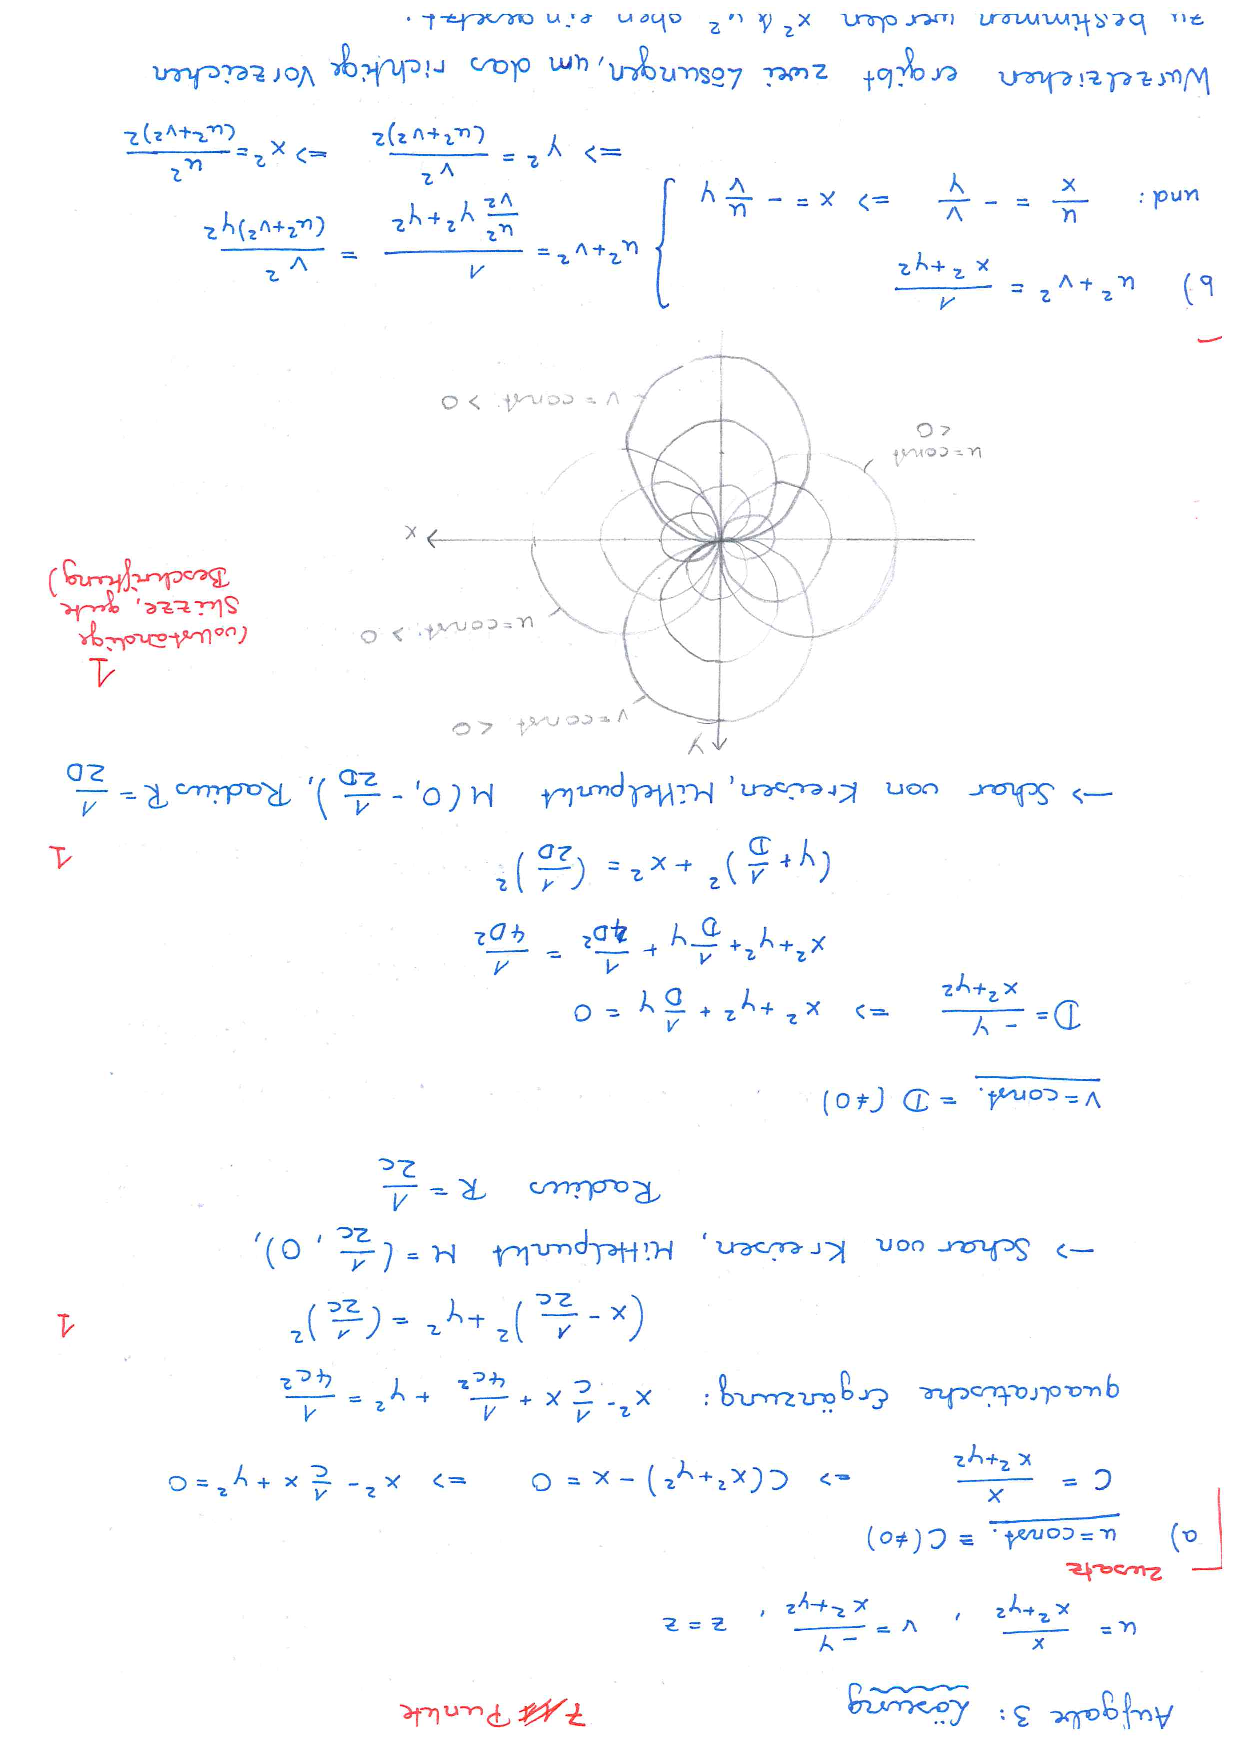
\includepdf[pages=-]{solution-krummlinig_vi.pdf}
  \end{atiSolution}
\end{document}